\documentclass[11pt]{article}

\usepackage{hyperref}
\usepackage{graphicx}
\usepackage{microtype}
\usepackage{xurl}
\usepackage{booktabs}
\usepackage{algorithm}
\usepackage{algpseudocode}
\usepackage{tikz}
\usetikzlibrary{automata,positioning,arrows.meta}

\title{Code-Owned Harnesses: Using System One Models for Bounded Agent Workflows}
\author{Ryan Martin}
\date{October 10, 2026}

\begin{document}
\maketitle

\begin{abstract}
Model-owned agent loops let the model choose the next tool and when to stop.
Each extra round spends more tokens, the path is hard to predict, and the model
is handed an open tool list. This paper describes a code-owned harness. A Rust
transition chooses the next step. System One models answer typed questions and
return probabilities and a confidence the machine can branch on. Generative
models run only inside an explicit node with a schema and a token cap, usually
after a gate. Effects run in Rust under a granted capability.
Section~\ref{sec:evaluation} quotes tokens, latency, and branch stability
for two fixtures against a ReAct-style baseline on the same generative model.
\end{abstract}

\section{Problem}
\label{sec:problem}

A common agent harness runs a loop until the model decides to stop. The model
sees a tool list, emits a call, receives the result, and chooses the next call.
Hermes centers that loop on one agent class that can write memory and create
skills~\cite{hermes-loop}. OpenClaw centers it on a gateway that loads skills
into the prompt and runs an embedded agent for the session~\cite{openclaw-loop}.
ReAct is the research form of the same idea: interleave reasoning traces with
actions~\cite{yao2023react}.

Three costs follow. Token spend grows with the number of rounds, and the model
chooses that number. The path is unpredictable, because the next tool is data
from the model rather than a branch in the program. Security is weak when the
same call can name any tool the process is allowed to run.

This paper inverts that arrangement. Code owns the next step. A System One
model answers a typed question and returns probabilities and a confidence.
A generative model is an escape hatch inside one schema-bounded node, usually
behind a gate. Effects run only after the host has granted a capability.
The implementation is a small Rust library~\cite{seaotter-agent}.

\section{Related work}
\label{sec:related}

Yao et al.\ introduce ReAct, which prompts a language model to alternate
between a reasoning trace and an action, and to stop when the model emits a
finish action~\cite{yao2023react}. The evaluation uses a ReAct-style loop on
the same generative model as its baseline.
Section~\ref{sec:evaluation} quotes the measured tokens, latency, and branch
stability.

Hermes and OpenClaw are production forms of a model-owned loop. Hermes
dispatches tools from an agent object, persists memory, and can create skills
during a run~\cite{hermes-loop}. OpenClaw loads a skills snapshot into the
prompt and executes tools inside a gateway-hosted agent
session~\cite{openclaw-loop}. Both treat the model's tool choice as control
flow.

The harness here keeps the model's output as data. The next node is a Rust
function. Confidence below a threshold takes an edge registered in code, or
the run halts. A generative call cannot select a tool, write memory, or name
the following step.

\section{Design}
\label{sec:design}

The next node is a transition. The machine stores the model output under the
node identifier and then applies
\begin{equation}
\delta : \mathit{Node} \times \mathit{Outcome} \times \mathit{State} \rightarrow \mathit{Next}.
\label{eq:delta}
\end{equation}
The output is a value. It is not a pointer to the next node.
Figure~\ref{fig:procedures} contrasts that step with a ReAct loop on the same
task.

A decision call sends only the state keys the node lists, plus a fixed set of
questions. A \texttt{Choice} question picks one label from a closed map. A
\texttt{Score} question ranks ordered levels. A \texttt{Noul} question is yes
or no. The response is a probability for each label and a confidence. If the
confidence is below the node's minimum, the machine skips the transition.
\texttt{SafeDefault}, \texttt{Escalate}, and \texttt{Human} go to handlers
registered on the workflow. \texttt{Continue} stays on the transition.
\texttt{RetryStronger} makes one further call to a second decision model and
then escalates if that call is still below the minimum. An action with no
handler halts the run.

A generative call is a separate node. It is one completion with a task, the
same kind of state slice, an output spec, and a token cap. The spec is a JSON
schema, or an explicit free-text opt-out. A gate usually sits in front of the
node. The model runs only when an earlier decision's top label matches the
allowed value and the confidence policy continued. A body that fails the
schema is rejected before the transition runs, so invalid text cannot choose
a node.

\begin{figure}[t]
\centering
\begin{minipage}[t]{0.48\textwidth}
\centering
\begin{algorithmic}[1]
\Procedure{ReAct}{$o$}
\For{$t \gets 1$ \textbf{to} $4$}
  \State $(thought, a) \gets complete(o)$
  \If{$a = \mathrm{finish}$}
    \State \Return branch
  \EndIf
\EndFor
\State \Return $\mathrm{unfinished}$
\EndProcedure
\end{algorithmic}
\end{minipage}\hfill
\begin{minipage}[t]{0.48\textwidth}
\centering
\begin{algorithmic}[1]
\Procedure{Harness}{$n, s$}
\State $x \gets \mathrm{slice}(s, \mathrm{reads}(n))$
\If{$n$ is Decide}
  \State $y \gets \mathrm{SystemOne}(x)$
\ElsIf{$n$ is Generate and the gate allows}
  \State $y \gets \mathrm{complete}(x)$
\EndIf
\State \Return $\delta(n, y, s)$
\EndProcedure
\end{algorithmic}
\end{minipage}
\caption{Control procedures. \textsc{ReAct} stops on $\mathrm{finish}$ or at
step four. \textsc{Harness} applies $\delta$ after one bounded model call.}
\label{fig:procedures}
\end{figure}

\section{Implementation}
\label{sec:implementation}

The library is three crates. \path{harness-core} holds the machine, the
node graph, the decision and generative traits, and the event log.
\path{harness-providers} supplies a System One decision client and
OpenAI-compatible and Anthropic generative clients. \path{harness-effects}
supplies the effects. Swapping the generative client does not change the
graph.

Effects run only when the machine has granted the matching capability.
\texttt{FileRead} is scoped to a path. \texttt{HttpGet} is scoped to an
allowlisted host. \texttt{DangerousShell} is off unless granted, and its
argument vector is fixed when Rust builds the effect. The node names the
effect. The model never receives a tool list, so it cannot name an effect,
invent a command, or write memory.

Every successful decide, generate, and effect step appends an event: the
node, the kind, a hash of the input, the output, an optional confidence, and
usage. A failed run returns the error and drops the log. Replay serves a
recorded step when the node, kind, and input hash match, and runs anything
else live. A diff of two runs reports path, output, and confidence
divergences.

Two examples fix the shapes used later for measurement.
\texttt{ticket-router} normalizes a ticket, asks a \texttt{Choice} over a
closed route set, and matches the top label in Rust. Low confidence takes a
safe-default queue. There is no generative call.
\texttt{gated-generate} asks a yes-or-no question. At sufficient confidence
the run reaches a draft node whose schema requires a string reply. A no
answer skips the model. Low confidence never visits the draft node.
Figure~\ref{fig:automata} is the state machine for each example.

\begin{figure}[t]
\centering
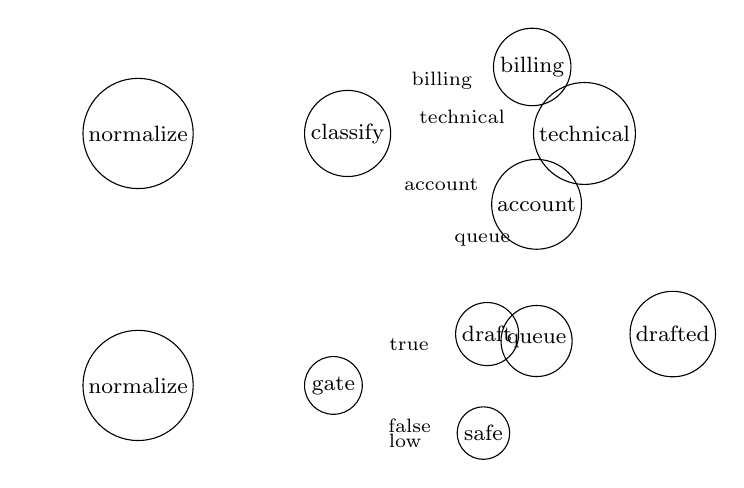
\begin{tikzpicture}[
  >=Stealth,
  shorten >=1pt,
  node distance=7mm and 14mm,
  every state/.style={font=\footnotesize, inner sep=1.5pt, minimum size=0pt},
  every edge/.style={font=\scriptsize},
  initial text={}
]
  \node[state, initial] (n) {normalize};
  \node[state, right=of n] (c) {classify};
  \node[state, above right=1mm and 16mm of c] (b) {billing};
  \node[state, right=18mm of c] (t) {technical};
  \node[state, below right=1mm and 16mm of c] (a) {account};
  \node[state, below=of a] (q) {queue};
  \path[->] (n) edge (c)
            (c) edge node[above] {billing} (b)
            (c) edge node[above] {technical} (t)
            (c) edge node[below] {account} (a)
            (c) edge node[right] {queue} (q);
  \begin{scope}[yshift=-32mm]
    \node[state, initial] (gn) {normalize};
    \node[state, right=of gn] (gg) {gate};
    \node[state, above right=1mm and 14mm of gg] (gd) {draft};
    \node[state, right=of gd] (gdd) {drafted};
    \node[state, below right=1mm and 14mm of gg] (gs) {safe};
    \path[->] (gn) edge (gg)
              (gg) edge node[above] {true} (gd)
              (gd) edge (gdd)
              (gg) edge node[below] {false} (gs)
              (gg) edge[bend right=15] node[below] {low} (gs);
  \end{scope}
\end{tikzpicture}
\caption{Measured automata. Low confidence in the ticket router takes
\texttt{queue}. A false or low-confidence gate takes \texttt{safe} and does
not call the generative model.}
\label{fig:automata}
\end{figure}

\section{Evaluation}
\label{sec:evaluation}

The baseline is a ReAct-style loop on the same OpenAI-compatible model the
harness uses for its generative draft, \path{gpt-4.1-mini-2025-04-14}.
Harness decisions use the System One model \texttt{jev-latest}.
Each ReAct step returns a thought and an action that matches a JSON schema.
The action \texttt{inspect} returns the fixture text.
The action \texttt{finish} ends the loop.
A loop that reaches four steps without finishing is branch \texttt{unfinished}.
Raw runs, the fixture paths, and the rerun command are in
\path{paper/measurements/}.
Ten runs of \path{examples/ticket-router/fixtures/billing.json} route one
support ticket.
Ten runs of \path{examples/gated-generate/fixtures/allow.json} decide whether
a reply may be drafted.
Table~\ref{tab:eval} reports the mean latency, token counts, and branch
stability.

\begin{table}[t]
\centering
\caption{Mean latency in milliseconds, input and output tokens, and branch
stability over ten runs.}
\label{tab:eval}
{\footnotesize
\begin{tabular}{@{}llrrrrr@{}}
\toprule
Workflow & Side & Branch & Stability & ms & Input & Output \\
\midrule
ticket router & harness & billing & 10/10 & 189.6 & 422.0 & 38.0 \\
ticket router & ReAct & billing & 10/10 & 1823.4 & 445.2 & 66.4 \\
gated generation & harness & safe & 10/10 & 200.1 & 296.0 & 20.0 \\
gated generation & ReAct & drafted & 10/10 & 2532.0 & 850.4 & 198.4 \\
\bottomrule
\end{tabular}}
\end{table}

\section{Limitations and future work}
\label{sec:limits}

Version~1 is a single-workflow library. It does not include a skill
marketplace, model-owned memory writes, multi-agent routing, a gateway, or an
open tool list. The model does not choose the next step.

The evaluation above is a micro-benchmark on two workflows.
It is not a field study of production tickets. Affiliation is omitted on this
title page and will be added before submission. Endorsement for a first arXiv
deposit is a submit-time step, not a result of this draft.

\section{Conclusion}
\label{sec:conclusion}

A code-owned harness spends model calls inside bounds the program sets.
System One is the default primitive: a typed answer and a confidence the
machine can branch on. A generative call remains available for prose or a
document, inside one gated node, with a schema. The next step stays a Rust
match.

\section*{Acknowledgments}

A language model helped draft the prose of this note. The author is
responsible for the content, including any errors.

\bibliographystyle{plain}
\bibliography{refs}

\end{document}
